%%%%%%%%%%%%%%%%%%%%%%%%%%%%%%%%%%%%%%%%%
% baposter Portrait Poster
% LaTeX Template
% Version 1.0 (15/5/13)
%
% Created by:
% Brian Amberg (baposter@brian-amberg.de)
%
% This template has been downloaded from:
% http://www.LaTeXTemplates.com
%
% License:
% CC BY-NC-SA 3.0 (http://creativecommons.org/licenses/by-nc-sa/3.0/)
%
%%%%%%%%%%%%%%%%%%%%%%%%%%%%%%%%%%%%%%%%%

%----------------------------------------------------------------------------------------
%	PACKAGES AND OTHER DOCUMENT CONFIGURATIONS
%----------------------------------------------------------------------------------------

\documentclass[a0paper,portrait]{baposter}
\usepackage[utf8]{inputenc}
\usepackage[brazilian]{babel}
\usepackage{verbatim, caption, subfig, array}
\usepackage{cite,url,amsthm,footmisc,bm}
\usepackage{amsmath,graphicx,amssymb,algorithm,algorithmic,graphicx,subfigure,epsfig,multirow,threeparttable,booktabs,bm,mathdots,tabularx}
\usepackage[font=small,labelfont=bf]{caption} % Required for specifying captions to tables and figures
\usepackage{booktabs} % Horizontal rules in tables
\usepackage{relsize} % Used for making text smaller in some places

\graphicspath{{figures/}} % Directory in which figures are stored

\definecolor{bordercol}{RGB}{40,40,40} % Border color of content boxes
\definecolor{headercol1}{RGB}{186,215,230} % Background color for the header in the content boxes (left side)
\definecolor{headercol2}{RGB}{130,130,130} % Background color for the header in the content boxes (right side)
\definecolor{headerfontcol}{RGB}{0,0,0} % Text color for the header text in the content boxes
\definecolor{boxcolor}{RGB}{255,255,255} % Background color for the content in the content boxes

\begin{document}

\background{ % Set the background to an image (background.pdf)
\begin{tikzpicture}[remember picture,overlay]
\draw (current page.north west)+(-2em,2em) node[anchor=north west]
{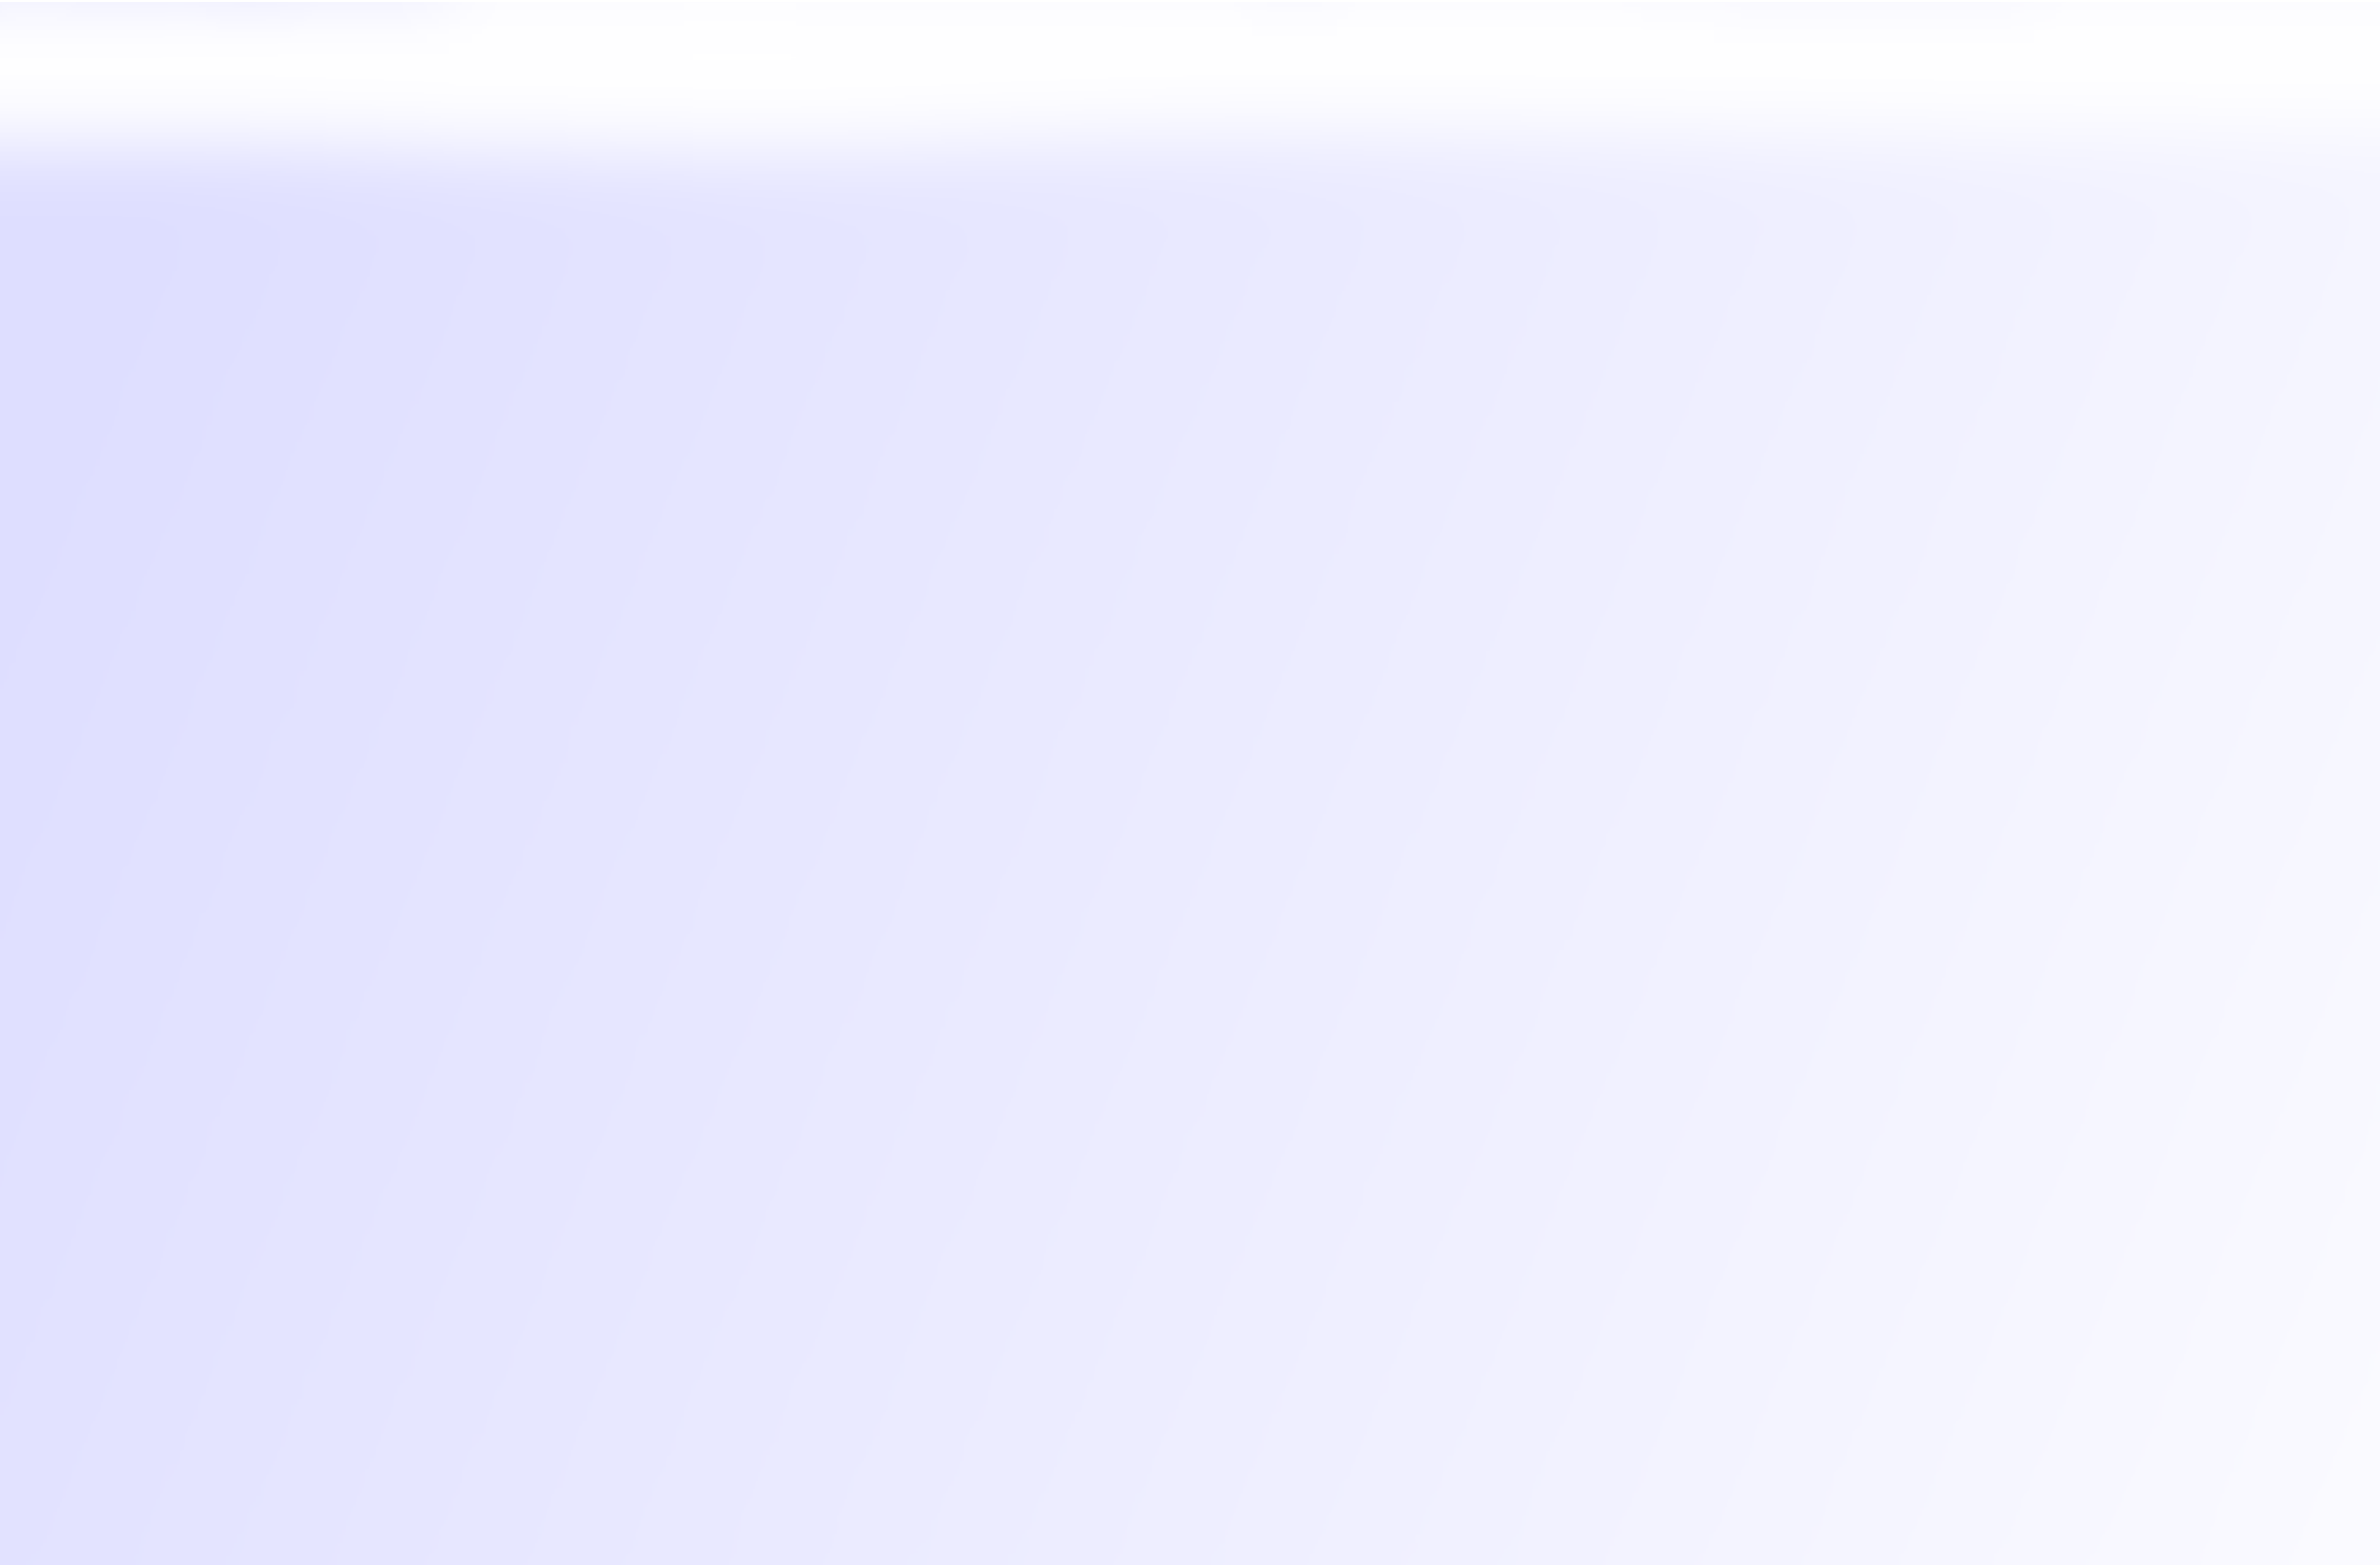
\includegraphics[height=1.1\textheight]{background}};
\end{tikzpicture}
}

\begin{poster}{
grid=false,
borderColor=bordercol, % Border color of content boxes
headerColorOne=headercol2, % Background color for the header in the content boxes (left side)
headerColorTwo=headercol1, % Background color for the header in the content boxes (right side)
headerFontColor=headerfontcol, % Text color for the header text in the content boxes
boxColorOne=boxcolor, % Background color for the content in the content boxes
headershape=roundedright, % Specify the rounded corner in the content box headers
headerfont=\Large\sf\bf, % Font modifiers for the text in the content box headers
textborder=rectangle,
background=user,
headerborder=open, % Change to closed for a line under the content box headers
boxshade=plain
}
{}
%
%----------------------------------------------------------------------------------------
%	TITLE AND AUTHOR NAME
%----------------------------------------------------------------------------------------
%
{\bf \huge \uppercase{Um estudo sobre o quarto elemento fundamental de circuitos: o  \emph{Memristor}}} % Poster title
{\vspace{1em} Cibelly Cristina, Lesly Montúfar e Yasmin Delbany\\ % Author names
{\smaller leslymontufar@ufu.br}} % Author email addresses
{
\includegraphics[width=2.5cm]{logo}} % University/lab logo

%----------------------------------------------------------------------------------------
%	INTRODUCTION
%----------------------------------------------------------------------------------------

\headerbox{Introdução}{name=introduction,column=0,row=0}{

A partir da análise das possíveis combinações entre as quatro variáveis fundamentais de circuitos: corrente elétrica $i$, tensão elétrica $v$, carga elétrica $q$ e fluxo magnético $\varphi$, Chua [1] 
%\cite{artigo}
 baseando-se no argumento da simetria, postulou que haveria um elemento de circuito faltante, capaz de associar a carga $q(t)$ e o fluxo magnético $\varphi(t)$. Por isso, em 1971, idealizou o novo componente, definido pela relação $d\varphi=M dq$, conforme a Figura \ref{memristor}, e denominou-o \emph{memristor}, uma contração de \emph{memory resistor}. 

\begin{center}
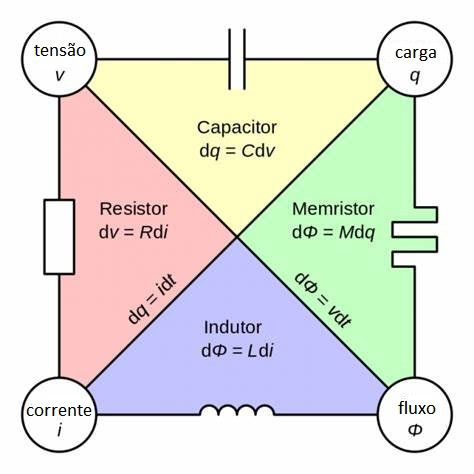
\includegraphics[width=0.8\linewidth]{memristor}
\vspace{-8pt}
\captionof{figure}{Combinação das quatro variáveis fundamentais de circuito.}
\label{memristor}
\end{center}

%, em português \emph{resistor com memória} 
Considerado, portanto, o quarto elemento fundamental dos circuitos eletrônicos, ao lado do capacitor (1745), resistor (1827) e indutor (1831), o \emph{memristor} destaca-se por apresentar uma propriedade da não-volatilidade, que, aliada a possibilidade de ser trabalhado em escala nanométrica, o torna promissor em aplicações como memórias ReRam e computação neuromórfica.


}

%----------------------------------------------------------------------------------------
%	MATERIALS AND METHODS
%----------------------------------------------------------------------------------------

\headerbox{Modelo de Deriva Linear}{name=methods,column=0,below=introduction}{
O primeiro modelo foi proposto pela \emph{HP Labs}

\begin{equation}
\begin{aligned}
\min_{\mathbf{S},\mathbf{W},\mathbf{F}}&\|\mathbf{S}-\mathbf{A}\|_F^2+\alpha\mathbf{Tr}(\mathbf{F}^T\mathbf{L_s}\mathbf{F})+\\&\beta(\|(\mathbf{XW}-\mathbf{F}\|_F^2+\gamma\|\mathbf{W}\|_{2,1}) \\
s.t.&~\mathbf{S1}=\mathbf{1},\mathbf{S}\ge\mathbf{0},\mathbf{F}^T\mathbf{F}=\mathbf{I}_c,\mathbf{F}\ge\mathbf{0}
\end{aligned}
\label{eq:3}
\end{equation}
where $\mathbf{X}\in\mathbb{R}^{n\times d}$ is the data matrix, $\mathbf{W}\in\mathbb{R}^{d\times c}$ is the projection matrix, $\beta$ and $\gamma$ are regularization parameters. Similar to [1, 2], we impose the non-negativity on F here
}

%----------------------------------------------------------------------------------------
%	CONCLUSION
%----------------------------------------------------------------------------------------

\headerbox{Conclusion}{name=conclusion,column=0,below=methods}{

Neste estudo, analisa-se os fundamentos físico-químicos e matemáticos do quarto elemento fundamental de circuitos: o \emph{memristor}. Idealizado por Chua em 1971, mas implementado apenas em 2008 pela \emph{HP Labs}, o novo componente tem o diferencial da propriedade de não-volatilidade, a qual é exemplificada mediante simulações nos ambientes \emph{MATLAB} e \emph{LTSPICE}, priorizando a explanação das características primeiro modelo proposto.

}

%----------------------------------------------------------------------------------------
%	REFERENCES
%----------------------------------------------------------------------------------------

\headerbox{References}{name=references,column=0,below=conclusion}{

\smaller % Reduce the font size in this block
\renewcommand{\section}[2]{\vskip 0.05em} % Get rid of the default "References" section title
\nocite{*} % Insert publications even if they are not cited in the poster

\bibliographystyle{unsrt}
\bibliography{sample} % Use sample.bib as the bibliography file
}

%----------------------------------------------------------------------------------------
%	ACKNOWLEDGEMENTS
%----------------------------------------------------------------------------------------



%----------------------------------------------------------------------------------------
%	RESULTS 1
%----------------------------------------------------------------------------------------

\headerbox{Funcionamento estrutural}{name=results1,span=2,column=1,row=0}{ % To reduce this block to 1 column width, remove 'span=2'
%\vspace{-15pt}

\begin{center}
\subfloat[]{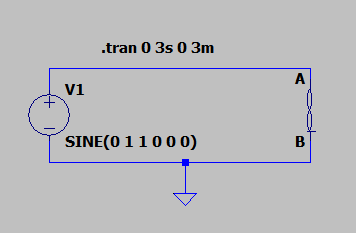
\includegraphics[width=0.45\linewidth]{ltspice}}\hfill
%\vspace{-8pt}
\subfloat[]{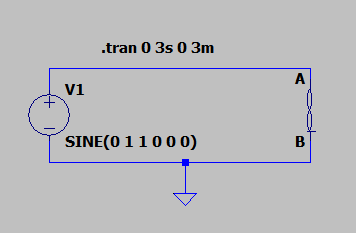
\includegraphics[width=0.45\linewidth]{ltspice}}
\vspace{-8pt}
\captionof{figure}{Performance of JGUFS algorithm for large variation of set of control parameters.} \label{ltspice:circuit}
\end{center}


}

%----------------------------------------------------------------------------------------
%	RESULTS 2
%----------------------------------------------------------------------------------------

\headerbox{Fundamentos Matemáticos}{name=results2,span=1,column=1,below=results1,above=bottom}{ % To reduce this block to 1 column width, remove 'span=2'
With other two variables fixed, the following formula can be proved: 
\begin{equation}\nonumber
\begin{aligned}
&\mathcal{O}(\mathbf{F}^{t+1}, \mathbf{W}^{t},\mathbf{S}^{t}) \leq \mathcal{O}(\mathbf{F}^{t}, \mathbf{W}^{t},\mathbf{S}^{t}), \\ &\mathcal{O}(\mathbf{F}^{t+1}, \mathbf{W}^{t+1},\mathbf{S}^{t}) \leq \mathcal{O}(\mathbf{F}^{t+1}, \mathbf{W}^{t},\mathbf{S}^{t}) \\ &\mathcal{O}(\mathbf{F}^{t+1}, \mathbf{W}^{t+1},\mathbf{S}^{t+1}) \leq \mathcal{O}(\mathbf{F}^{t+1}, \mathbf{W}^{t+1},\mathbf{S}^{t})
\end{aligned}
\end{equation}

We conclude that JGUFS objective function monotonically decreases under the optimization in Algorithm. 1.

\begin{algorithm}[H]
  \renewcommand{\algorithmicrequire}{\textbf{Input:}}
  \renewcommand{\algorithmicensure}{\textbf{Output:}}
  \caption{Optimization to JGUFS objective function}
    \begin{algorithmic}[1]
    \REQUIRE Data matrix $\mathbf{X}\in\mathbb{R}^{n\times d}$, $\lambda$, $\beta$, and $\gamma$, $c$, the dimension of projected subspace c;
    \ENSURE Rank features based on the values of $\|w_i\|_2|_{i=1}^d$ in descending order and then select the top-ranked ones.
    \STATE Initialization. Construct the initial graph affinity matrix $\mathbf{A}$ based on the 'HeatKernel' function; Calculate $\mathbf{F}\in\mathbb{R}^{n\times c}$ by the c eigenvectors of the graph Laplacian $\mathbf{L_A}=\mathbf{D_A}-\frac{\mathbf{A}^T+\mathbf{A}}{2}$ corresponding to the c smallest eigenvalues; Initialize $\mathbf{M}\in\mathbb{R}^{d\times d}$ as an identity matrix;;
    \WHILE {not converged}
    \STATE Update $\mathbf{S}$ by solving:
    \vspace{-10pt}
    \begin{equation}\nonumber
        \min_{S_i\mathbf{1}=1,s_i\ge0}\|s_i-(a_i-\frac{\alpha}{2}d_i)\|_F^2,
    \end{equation}
    
    where, $d_{ij}=\|f_i-f_j\|_2^2$ and $d_i$ as a vector with the $j$-th element equal to $d_{ij}$. Similarly, we get $a_i$ and $s_i$.
    \STATE Update $\mathbf{W}$ by:
    \vspace{-7pt}
    \begin{equation}\nonumber
       \mathbf{W}=(\mathbf{X}^T\mathbf{X}+\gamma\mathbf{M})^{-1}\mathbf{X}^T\mathbf{F}
    \end{equation}
    \vspace{-15pt}
    \STATE Update $\mathbf{M}$ by:
    \vspace{-7pt}
    \begin{equation}\nonumber
        m_{ii}=\frac{1}{2\|w\|_2}=\frac{1}{2\sqrt{w_iw_i^T+\delta}}
    \end{equation}
    \vspace{-10pt}
    \STATE Update $\mathbf{F}$ by:
    \vspace{-10pt}
    \begin{equation}\nonumber
        d_{ij} \leftarrow \frac{(\lambda \mathbf{F})_{ij}}{\mathbf{R}\mathbf{F}+\lambda\mathbf{FF}^T\mathbf{F}}
    \end{equation}
    \vspace{-15pt}
    \ENDWHILE
    \end{algorithmic}
    \label{alg:1}
\end{algorithm}

%------------------------------------------------

}

%----------------------------------------------------------------------------------------
---
%	RESULTS 2
%----------------------------------------------------------------------------------------

\headerbox{Análise computacional}{name=results2,span=1,column=2,below=results1,above=bottom}{ % To reduce this block to 1 column width, remove 'span=2'
As Figuras \ref{ltspice:circuit}, \ref{ltspice:tempo} e \ref{ltspice:pinched}, obtidas pelo simulador \emph{LTSPICE}, ilustra o seguinte teorema fundamental: "todo dispositivo de duplo terminal que exibe um \emph{pinched hysteresis loop} no plano tensão-corrente quando conduzido por um sinal DC e/ou senoidal de qualquer frequência é um sistema memristivo".

\vspace{-5pt}
%------------------------------------------------

\begin{center}
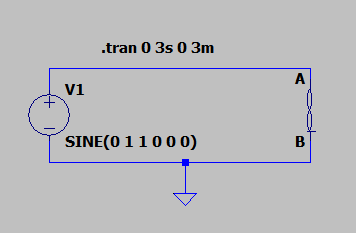
\includegraphics[width=0.8\linewidth]{ltspice}
\vspace{-8pt}
\captionof{figure}{Performance of JGUFS algorithm for large variation of set of control parameters.} \label{ltspice:circuit}
\end{center}

%------------------------------------------------
\vspace{-15pt}
\begin{center}
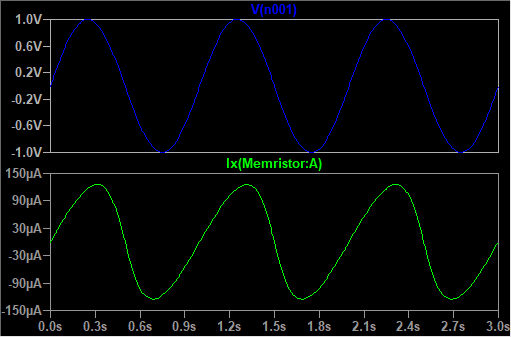
\includegraphics[width=0.8\linewidth]{vt-it}
\vspace{-8pt}
\captionof{figure}{Convergence speed of JGUFS for UMIST and COIL20 data sets.} \label{ltspice:tempo}
\end{center}

%------------------------------------------------
\vspace{-15pt}
\begin{center}
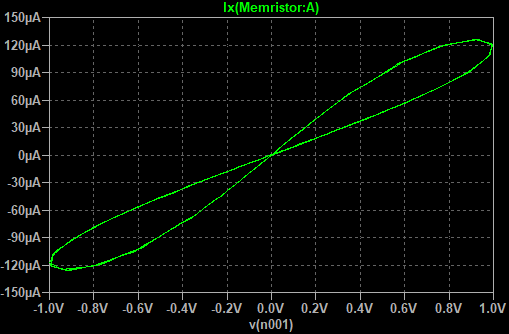
\includegraphics[width=0.8\linewidth]{pinched}
\vspace{-8pt}
\captionof{figure}{Convergence speed of JGUFS for UMIST and COIL20 data sets.}\label{ltspice:pinched}
\end{center}

%------------------------------------------------
\vspace{-8pt}
 


}

\end{poster}

\end{document}